\documentclass[12pt,a4paper]{report}

\usepackage[margin=1in]{geometry}
\usepackage{graphicx}
\usepackage{array}
\usepackage{booktabs}
\usepackage{float}
\usepackage{setspace}
\usepackage{titlesec}
\usepackage{tocloft}
\usepackage{enumitem}
\usepackage{hyperref}
\usepackage{xcolor}
\usepackage{url}
\usepackage{eso-pic}
\usepackage{tikz}
\usepackage{fancyhdr}
\usepackage{lastpage}
\usepackage{etoolbox}

\hypersetup{
    colorlinks=true,
    linkcolor=black,
    urlcolor=blue,
    pdftitle={Internship Report},
    pdfauthor={Keerthana C}
}

% -- Spacing ----------------------------------------------------------------
\setstretch{1.5}
\setlength{\parindent}{1.5em}
\setlength{\parskip}{0.4em}

% -- Chapter heading format -------------------------------------------------
\titleformat{\chapter}[display]
  {\filcenter\bfseries\Large}
  {\chaptername~\thechapter}{10pt}{\LARGE\markboth{\MakeUppercase{##1}}{\MakeUppercase{##1}}}

% Ensure chapter marks are set for headers
\renewcommand{\chaptermark}[1]{\markboth{##1}{##1}}

% -- Rename TOC / LOF headings to match template ----------------------------
\renewcommand{\contentsname}{TABLE OF CONTENTS}
\renewcommand{\listfigurename}{LIST OF FIGURES}

% -- TOC heading format (consistent with other front-matter headings) -------
\renewcommand{\cfttoctitlefont}{\hfill\LARGE\bfseries}
\renewcommand{\cftaftertoctitle}{\hfill}
\renewcommand{\cftloftitlefont}{\hfill\LARGE\bfseries}
\renewcommand{\cftafterloftitle}{\hfill}
\setlength{\cftbeforetoctitleskip}{-1.5em}
\setlength{\cftaftertoctitleskip}{1.5em}
\setlength{\cftbeforeloftitleskip}{-1.5em}
\setlength{\cftafterloftitleskip}{1.5em}
\renewcommand{\cftsecleader}{\cftdotfill{\cftdotsep}}
\renewcommand{\cftchapleader}{\cftdotfill{\cftdotsep}}

% -- Toggle: border ON/OFF --------------------------------------------------
% We define a boolean that controls whether borders are drawn.
% Front-matter pages: border ON.  Chapter pages: border OFF.
\newif\ifshowborder
\showbordertrue  % start with borders ON

\AddToShipoutPictureBG{%
  \ifshowborder
  \begin{tikzpicture}[remember picture, overlay]
    \draw[line width=0.56pt]
      ([xshift=18pt, yshift=-18pt]current page.north west)
      rectangle
      ([xshift=-18pt, yshift=18pt]current page.south east);
    \draw[line width=0.28pt]
      ([xshift=20pt, yshift=-20pt]current page.north west)
      rectangle
      ([xshift=-20pt, yshift=20pt]current page.south east);
  \end{tikzpicture}%
  \fi
}

% -- Page styles ------------------------------------------------------------

% Style for front-matter: no header/footer, just centered page number
\fancypagestyle{frontmatter}{
  \fancyhf{}
  \renewcommand{\headrulewidth}{0pt}
  \renewcommand{\footrulewidth}{0pt}
  \fancyfoot[C]{\thepage}
}

% Style for main content: header + footer, no border
\fancypagestyle{mainchapter}{
  \fancyhf{}
  \renewcommand{\headrulewidth}{0.4pt}
  \renewcommand{\footrulewidth}{0.4pt}
  \fancyhead[L]{\small Developer}
  \fancyhead[R]{\small\nouppercase{\leftmark}}
  \fancyfoot[L]{\small Dept. of ECE, Vemana IT}
  \fancyfoot[C]{\small 2025-2026}
  \fancyfoot[R]{\small Page \thepage\ of \pageref{LastPage}}
  \renewcommand{\chaptermark}[1]{\markboth{##1}{}}
}

% Plain style for front-matter (used by \chapter*, \listoffigures, etc.)
% Initially just centered page number. Redefined before main content.
\fancypagestyle{plain}{
  \fancyhf{}
  \renewcommand{\headrulewidth}{0pt}
  \renewcommand{\footrulewidth}{0pt}
  \fancyfoot[C]{\thepage}
}

\begin{document}

% ==========================================================================
% TITLE PAGE  (single-spaced, zero parskip so it fits on one page)
% ==========================================================================
\begin{titlepage}
\thispagestyle{empty}
\begin{singlespacing}
\setlength{\parskip}{0pt}
\setlength{\parindent}{0pt}
\centering
\vspace*{-0.5cm}

{\Large \textbf{VISVESVARAYA TECHNOLOGICAL UNIVERSITY}\par}
\vspace{2pt}
{\large \textbf{Jnana Sangama, Belagavi -- 590018}\par}
\vspace{8pt}

\includegraphics[height=5cm]{images/vtu_logo.png}\par
\vspace{8pt}
{\itshape An Internship Report\par}
\vspace{2pt}
{\itshape On\par}
\vspace{4pt}
{\LARGE \textbf{\textquotedblleft Developer\textquotedblright}\par}
\vspace{4pt}
{\textcolor{red}{Feb 2 to May 2}\par}
\vspace{8pt}
{\itshape Submitted in partial fulfillment of the requirements for the award of the degree of\par}
\vspace{4pt}
{\large \textbf{Bachelor of Engineering}\par}
\vspace{2pt}
{\large \textbf{in}\par}
\vspace{2pt}
{\large \textbf{\textcolor{blue}{Electronics and communication Engineering}}\par}
\vspace{8pt}
Submitted by\par
\vspace{4pt}
{\large \textbf{KEERTHANA C \hspace{2cm} 1VI22EC072}\par}
\vspace{10pt}

\includegraphics[height=4cm]{images/vit_logo.png}\par
\vspace{10pt}
{\large \textbf{DEPARTMENT OF ELECTRONICS AND COMMUNICATION ENGINEERING}\par}
{\Large \textbf{VEMANA INSTITUTE OF TECHNOLOGY}\par}
{\large BENGALURU -- 560034\par}
\vspace{6pt}
{\Large \textbf{2025-2026}\par}

\end{singlespacing}
\end{titlepage}

% ==========================================================================
% FRONT MATTER — borders ON, roman numbering, no headers/footers
% ==========================================================================
\pagenumbering{roman}
\pagestyle{frontmatter}

% ==========================================================================
% CERTIFICATE PAGE
% ==========================================================================
\thispagestyle{empty}
\begin{singlespacing}
\setlength{\parskip}{0pt}
\setlength{\parindent}{0pt}
\begin{center}
{\large \textbf{Karnataka ReddyJana Sangha}\par}
\vspace{2pt}
{\Large \textbf{VEMANA INSTITUTE OF TECHNOLOGY}\par}
\vspace{2pt}
(Affiliated to Visvesvaraya Technological University, Belagavi)\par
Koramangala, Bengaluru--560034\par
\vspace{8pt}

\includegraphics[height=3.5cm]{images/dept_seal.png}\par
\vspace{10pt}
{\large \textbf{DEPARTMENT OF}\par}
{\large \textbf{ELECTRONICS AND COMMUNICATION ENGINEERING}\par}
\vspace{10pt}
\addcontentsline{toc}{chapter}{Certificate}
{\LARGE \textbf{CERTIFICATE}\par}
\end{center}
\end{singlespacing}

\vspace{6pt}
\setlength{\parindent}{1.5em}
This is to certify that the internship entitled \textbf{\textquotedblleft Developer\textquotedblright} is a bonafide work carried out by \textbf{KEERTHANA C (1VI22EC072)} in partial fulfilment of the requirements for the award of Bachelor of Engineering degree in \textbf{Electronics and communication Engineering}, Visvesvaraya Technological University, Belagavi, during the academic year 2025-2026.

It is certified that all corrections and suggestions indicated for internal assessment have been duly incorporated in the report. The internship report has been approved as it satisfies the academic requirements prescribed for the said degree.

% -- Watermark: VIT logo behind signatures ---------------------------------
\AddToShipoutPictureFG*{%
  \begin{tikzpicture}[remember picture, overlay]
    \node[opacity=0.10] at ([yshift=-4cm]current page.center) {%
      
\includegraphics[height=8cm]{images/vit_logo.png}%
    };
  \end{tikzpicture}%
}

\vspace{0.6cm}
\begin{center}
\begin{tabular}{>{\raggedright\arraybackslash}p{0.23\textwidth} >{\raggedright\arraybackslash}p{0.24\textwidth} >{\raggedright\arraybackslash}p{0.20\textwidth} >{\raggedright\arraybackslash}p{0.23\textwidth}}
\textbf{Internal Supervisor} & \textbf{External Supervisor} & \textbf{HOD} & \textbf{Principal} \\
(Prof. Suma B V) & (N. Vijay Anand) & (Dr. Suneeta) & (Dr. Vijayasimha Reddy B G) \\
\end{tabular}
\end{center}

\vspace{0.5cm}
\textbf{Name of the Examiners} \hfill \textbf{Signature with Date}\par
\vspace{0.2cm}
1.\enspace\rule{5cm}{0.4pt} \hfill \rule{3.5cm}{0.4pt}\par
\vspace{0.4cm}
2.\enspace\rule{5cm}{0.4pt} \hfill \rule{3.5cm}{0.4pt}\par


\newpage
\begin{center}
\vspace*{\fill}
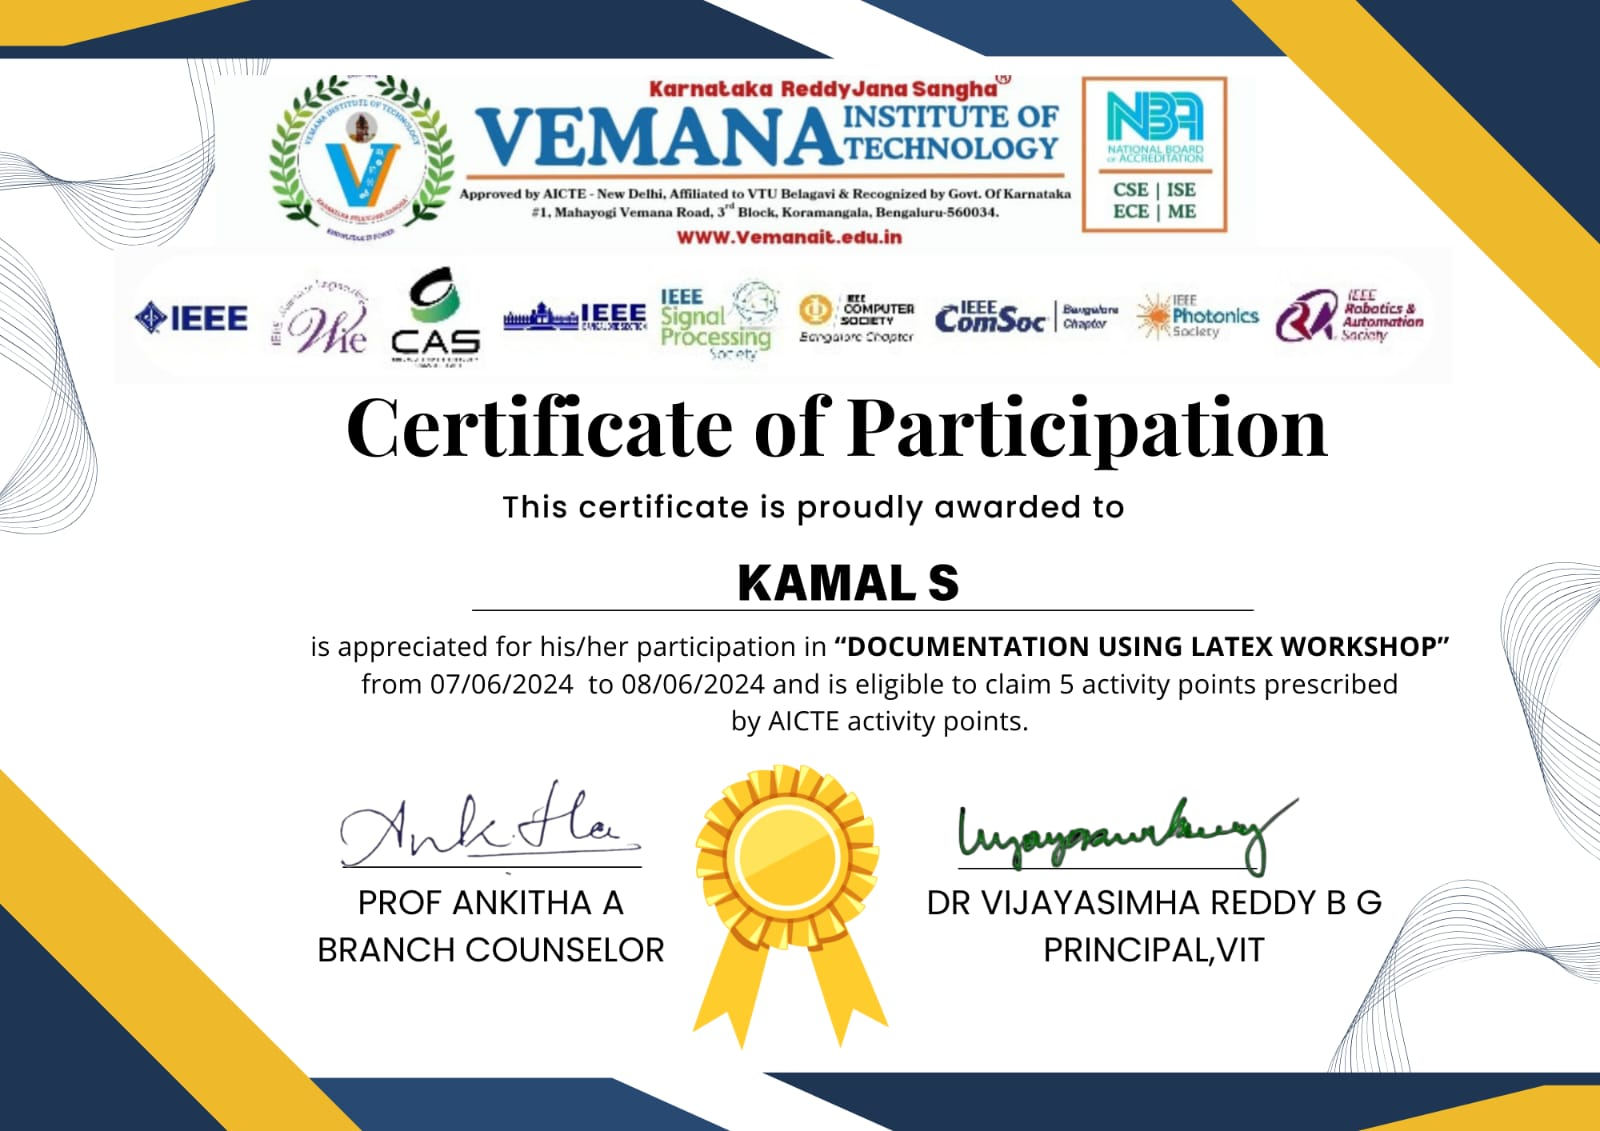
\includegraphics[angle=90,origin=c,width=0.92\textheight,height=0.92\textwidth,keepaspectratio]{images/cert_image_9c7970f1.jpeg}
\vspace*{\fill}
\end{center}


% ==========================================================================
% ACKNOWLEDGEMENT
% ==========================================================================
\newpage
\setcounter{page}{2}  % Ack = page ii (certificate was empty)
\begin{center}
{\LARGE \textbf{ACKNOWLEDGEMENT}\par}
\end{center}
\addcontentsline{toc}{chapter}{Acknowledgement}

\vspace{0.5cm}
\setlength{\parskip}{1em}
\begin{onehalfspacing}
I sincerely thank Visvesvaraya Technological University (VTU) for providing me with the opportunity to undertake this internship as a part of the academic curriculum, which has contributed significantly to my learning and overall development.

I express my sincere gratitude to 	extbf{Dr. Vijayasimha Reddy B G}, Principal, Vemana Institute of Technology, Bengaluru, for providing the necessary infrastructure, encouragement, and support to successfully carry out the internship work.

I extend my heartfelt thanks to 	extbf{Dr. Suneeta}, Head of the Department, Electronics and communication Engineering, Vemana Institute of Technology, for their constant guidance, motivation, and encouragement throughout the internship duration.

I would also like to thank Internal Supervisor 	extbf{Prof. Suma B V}, External Supervisor 	extbf{N. Vijay Anand}, and all Internship Coordinators for their cooperation, coordination, and support during the internship period.

I am thankful to all the teaching and non-teaching staff members of the Department of Electronics and communication Engineering for their support and encouragement throughout the internship.

I also acknowledge the support of 	extbf{TriSpace} for providing structured learning resources and an environment that encouraged systematic understanding, practical application, and continuous improvement.
\end{onehalfspacing}
\setlength{\parskip}{0.4em}

\vspace{1cm}
\begin{flushright}
\textbf{Keerthana C}\par
1VI22EC072\par
\end{flushright}

% ==========================================================================
% ABSTRACT
% ==========================================================================
\newpage
\begin{center}
{\LARGE \textbf{ABSTRACT}\par}
\end{center}
\addcontentsline{toc}{chapter}{Abstract}

\vspace{0.5cm}
\setlength{\parindent}{1.5em}

Abstract not provided.


% ==========================================================================
% TABLE OF CONTENTS — Standard LaTeX TOC with dotted leaders
% ==========================================================================
\newpage
\tableofcontents

% ==========================================================================
% LIST OF FIGURES — Custom table format matching template
% ==========================================================================
\newpage
% We need the custom header for LOF
\addtocontents{lof}{\textbf{Figure No} \hfill \textbf{Title} \hfill \textbf{Page No}\par\smallskip\hrule\par\bigskip}
\listoffigures

% ==========================================================================
% MAIN CONTENT — borders OFF, headers/footers ON, arabic numbering
% ==========================================================================
\newpage
\showborderfalse       % TURN OFF borders for all remaining pages
\pagenumbering{arabic}

% Redefine plain style for chapter first pages — SAME as mainchapter
% Template shows header + footer on ALL chapter pages including the first page
\fancypagestyle{plain}{
  \fancyhf{}
  \renewcommand{\headrulewidth}{0.4pt}
  \renewcommand{\footrulewidth}{0.4pt}
  \fancyhead[L]{\small Developer}
  \fancyhead[R]{\small\nouppercase{\leftmark}}
  \fancyfoot[L]{\small Dept. of ECE, Vemana IT}
  \fancyfoot[C]{\small 2025-2026}
  \fancyfoot[R]{\small Page \thepage\ of \pageref{LastPage}}
  \renewcommand{\chaptermark}[1]{\markboth{##1}{}}
}
\pagestyle{mainchapter}

% ==========================================================================
% CHAPTER 1: INTRODUCTION
% ==========================================================================
\chapter{INTRODUCTION}
\label{ch:intro}


This chapter provides an introduction to my internship experience at TriSpace in the role of Developer. It outlines the objectives, scope, and relevance of the internship in relation to my academic background in Electronics and communication Engineering. The chapter also discusses the evolution of technologies and current trends related to the work carried out during the internship period. Internships play a crucial role in bridging the gap between theoretical knowledge gained in the classroom and practical skills required in the industry. This internship provided me with a unique opportunity to apply my engineering knowledge in a real-world professional environment, working alongside experienced professionals and contributing to meaningful projects.


\section{Internship Scope and Objectives}


\section{Relevance of Developer to Electronics and communication Engineering}


\section{Evolution of Practices in the Field}


\section{Current Trends and Technologies}




% ==========================================================================
% CHAPTER 2: ORGANISATION PROFILE
% ==========================================================================
\chapter{ORGANISATION PROFILE}
\label{ch:org}


In addition to answering questions like when and where the internship was completed, this chapter gives a comprehensive overview of TriSpace and concentrates on its history, founding vision, organizational structure, services offered, and overall impact in the industry. Understanding the organization where the internship was carried out is essential as it provides context for the work done and helps in appreciating the learning environment that contributed to the overall internship experience.


\section{Introduction}

TriSpace is a leading organization that provides structured learning, training, and internship programs to engineering students and professionals across multiple domains. The organization has established itself as a reputable entity in the technology sector, known for fostering innovation, supporting skill development, and contributing to the growth of the engineering workforce. With a commitment to practical education and industry-aligned training, the organization has been instrumental in shaping the careers of numerous students and professionals.



\begin{figure}[H]
\centering

\includegraphics[width=0.55\textwidth,height=5cm,keepaspectratio]{images/company_logo_f66fab2d.png}
\caption{Internship Provider - TriSpace Logo}
\end{figure}


\section{Vision and Mission of the Organization}


\section{Programs and Services Offered}


\section{Organizational Impact and Reach}


\section{Core Values}



\begin{figure}[H]
\centering
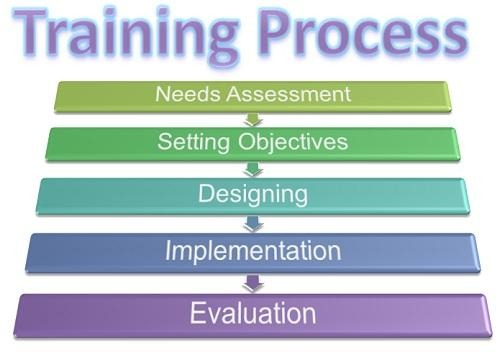
\includegraphics[width=0.45\textwidth,height=5cm,keepaspectratio]{images/ch_img_06a83fac.jpeg}
\caption{training process}
\end{figure}


% ==========================================================================
% CHAPTER 3: WORK DONE / METHODOLOGY
% ==========================================================================
\chapter{WORK DONE / METHODOLOGY}
\label{ch:work}


The work completed during the internship and the methodology used are presented in this chapter. This chapter provides a detailed account of the day-to-day activities, the tools and technologies employed, the work process followed, and the key projects undertaken. It also discusses the challenges encountered during the internship and the solutions implemented to overcome them. The chapter aims to give a comprehensive understanding of the practical work experience gained during the internship period.


\section{Overview of Internship Work}


\section{Tools and Technologies Used}



\begin{figure}[H]
\centering
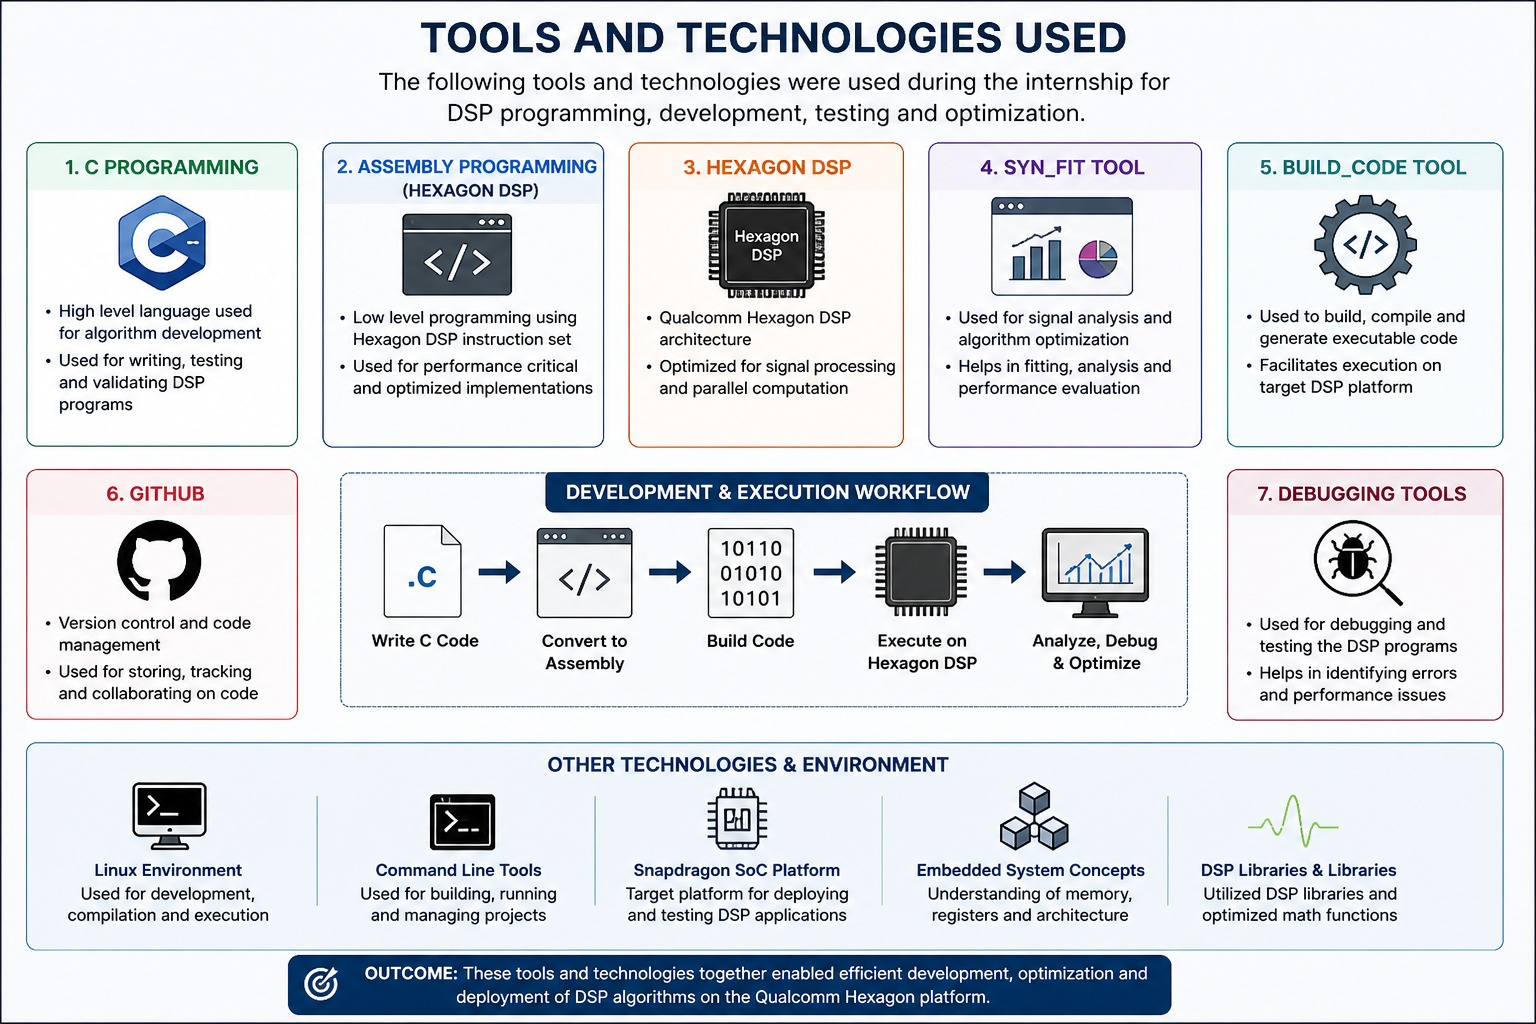
\includegraphics[width=0.45\textwidth,height=5cm,keepaspectratio]{images/ch_img_608851ac.jpeg}
\caption{Tools and technologies}
\end{figure}


\begin{figure}[H]
\centering
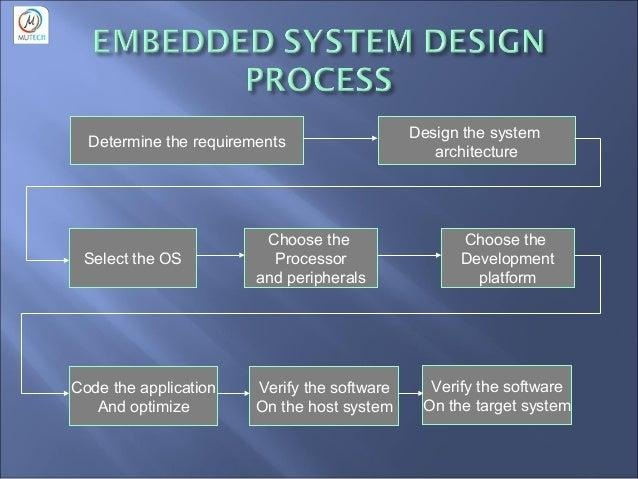
\includegraphics[width=0.45\textwidth,height=5cm,keepaspectratio]{images/ch_img_d5fed2bd.jpeg}
\caption{Embedded system design process}
\end{figure}


\section{Work Process and Methodology}


\section{Key Project and Case Study}




\section{Challenges Faced}


\section{Solutions Implemented}


% ==========================================================================
% CHAPTER 4: RESULTS AND DISCUSSION
% ==========================================================================
\chapter{RESULTS AND DISCUSSION}
\label{ch:results}


The work that was evaluated and examined during the internship is included in this chapter. This chapter presents a thorough analysis of the outcomes achieved, the learning acquired, and the overall effectiveness of the internship experience. It evaluates the deliverables produced, the skills developed, and provides a critical analysis of the entire internship journey, highlighting both the successes and areas for improvement.



\begin{figure}[H]
\centering
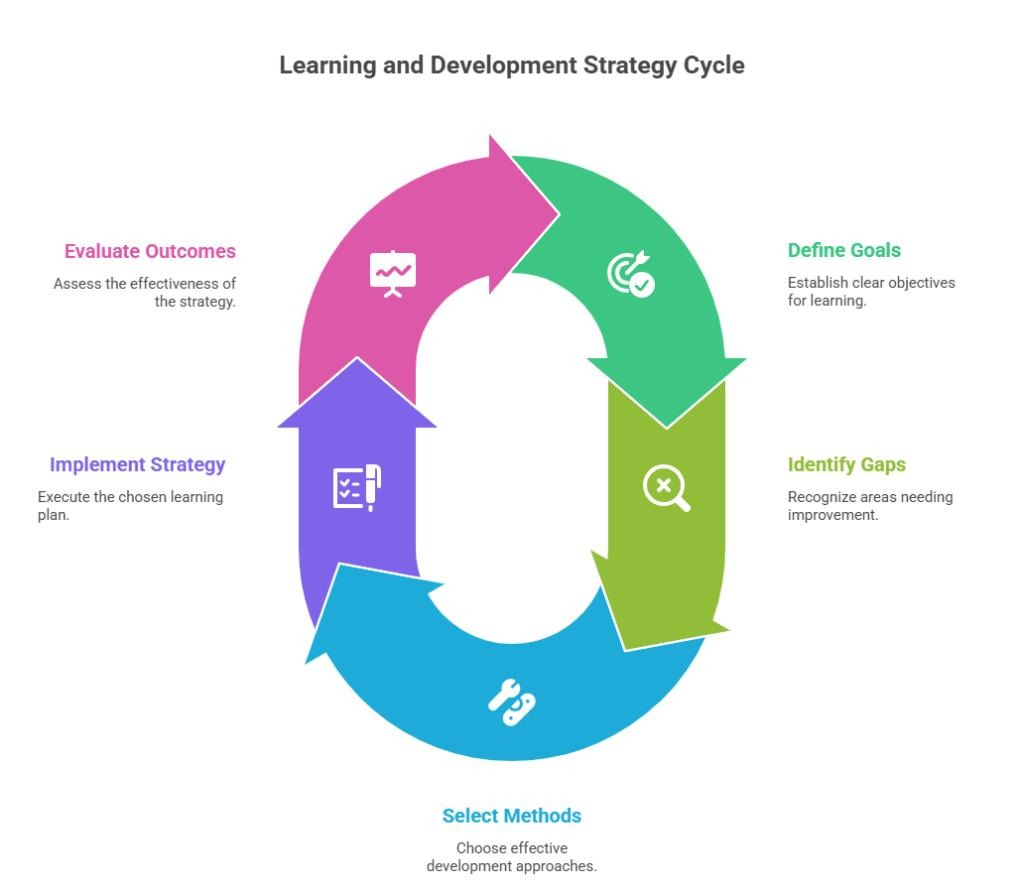
\includegraphics[width=0.45\textwidth,height=5cm,keepaspectratio]{images/ch_img_b83ab52c.jpeg}
\caption{Learning and Development Strategy Cycle}
\end{figure}


\section{Outcomes of the Work}


\section{Learning Outcomes}


\section{Analysis}




% ==========================================================================
% CHAPTER 5: CONCLUSION
% ==========================================================================
\chapter{CONCLUSION}
\label{ch:conclusion}


This chapter summarizes the overall internship experience, highlighting key outcomes, personal growth, and future directions.




\section{Summary}


\section{Personal Growth}


\section{Future Scope}


\end{document}
